\documentclass[aspectratio=169,11pt]{beamer}

\usetheme{CambridgeUS}
\usecolortheme{seahorse}
\useinnertheme{rectangles}
\useoutertheme{infolines}
\setbeamertemplate{navigation symbols}{}
\setbeamertemplate{footline}[frame number]

\usepackage[utf8]{inputenc}
\usepackage{graphicx}
\usepackage{booktabs}
\usepackage{amsmath}
\usepackage{hyperref}

\graphicspath{{./}{plots/}{report_diagrams/}{sla_plots/}}

\title[Annual Progress]{Utilizing Satellite-Based Observations to Correct the CMIP6 Climate Projections of Sea Level Anomaly and Significant Wave Height}
\subtitle{Annual Progress Presentation (Year 1: 01 Mar 2025 -- 28 Feb 2026)}
\author{Pritam Anand (PI) \and Shyam Saktawat (JRF)}
\institute{DA-IICT, Gandhinagar, India}
\date{}

\begin{document}

\begin{frame}
  \titlepage
\end{frame}

\begin{frame}{Agenda}
  \tableofcontents
\end{frame}

\section{Introduction}

\begin{frame}{Introduction}
  \begin{itemize}
    \item Sea level anomaly (SLA) and significant wave height (SWH) are core variables for coastal risk, engineering design, and climate services.
    \item CMIP6 provides historical and future projections under Shared Socioeconomic Pathways (SSPs), but biases limit direct usability for decision-making.
    \item Satellite altimetry provides a consistent multi-mission observational baseline to quantify and correct model biases.
    \item Goal: develop a scalable, reproducible correction workflow that yields corrected products and uncertainty information for dissemination.
  \end{itemize}
\end{frame}

\section{Research Problem and Objectives}

\begin{frame}{Research Problem}
  \begin{itemize}
    \item Earth System Models can show systematic errors due to parameterizations, grid resolution, and incomplete representation of ocean--atmosphere processes.
    \item Biases in SLA and SWH can propagate into errors in coastal hazard assessments, adaptation planning, and infrastructure design.
    \item Need: quantify uncertainty and build data-driven corrections using a reliable observational reference.
  \end{itemize}
  \vspace{0.75em}
  \textbf{Objectives}
  \begin{itemize}
    \item Quantify uncertainties in CMIP6 SWH and SLA (2015--2023 overlap) against merged satellite altimetry.
    \item Develop AI/ML bias-correction models (pilot Random Forest; planned probabilistic models) to reduce systematic errors.
    \item Produce corrected datasets (NetCDF) with uncertainty layers, targeting dissemination through MOSDAC.
  \end{itemize}
\end{frame}

\section{Literature Review}

\begin{frame}{Literature Review (Selected)}
  \begin{itemize}
    \item Bias correction for wave climate and ocean variables is widely recognized as necessary before using projections for impacts.
    \item Traditional approaches: quantile mapping and multivariate extensions to correct distributions and dependencies.
    \item ML approaches: Random Forest and deep learning can learn spatially varying, nonlinear correction mappings.
    \item Probabilistic forecasting: models such as DeepAR and Bayesian/ensemble methods provide prediction intervals for uncertainty-aware products.
  \end{itemize}
\end{frame}

\section{Methodology}

\begin{frame}{Datasets}
  \begin{itemize}
    \item \textbf{Observations:} CMEMS/AVISO DUACS Level-4 gridded products (SLA; SWH where applicable), multi-mission merged, global coverage.
    \item \textbf{Models:} CMIP6 variables including SWH and sea surface height (\texttt{zos}) from ESGF.
    \item \textbf{Pilot domains:}
      \begin{itemize}
        \item SWH: Indian Ocean sector (50--110$^\circ$E, 70$^\circ$S--70$^\circ$N), 2015--2020 overlap.
        \item SLA: high-latitude pilot region to validate robustness under complex coast/ice conditions.
      \end{itemize}
  \end{itemize}
\end{frame}

\begin{frame}{Preprocessing and Harmonization}
  \begin{itemize}
    \item Quality control, dynamic ocean masking, and handling of missing values.
    \item Monthly time alignment to match CMIP6 ocean output frequency.
    \item Regridding/co-location to a common grid (bilinear/conservative as appropriate; nearest-neighbour for curvilinear grids in SLA pilot).
    \item SLA anomaly computation by removing long-term mean reference from \texttt{zos}.
  \end{itemize}
\end{frame}

\begin{frame}{Bias Correction Modeling}
  \begin{columns}[T,onlytextwidth]
    \column{0.52\textwidth}
      \textbf{Pilot baseline model}
      \begin{itemize}
        \item Random Forest regressor to learn the mapping: CMIP6 $\rightarrow$ satellite reference.
        \item Features (pilot): CMIP6 value, latitude, longitude, month/seasonality.
        \item Target: satellite-observed SWH or SLA on aligned grid.
      \end{itemize}
      \vspace{0.5em}
      \textbf{Validation}
      \begin{itemize}
        \item Metrics: RMSE, MAE, $R^2$, correlation.
        \item Spatial/temporal splitting (pilot demonstration).
      \end{itemize}
    \column{0.48\textwidth}
      \centering
      
\includegraphics[width=\textwidth]{model_schema.png}
  \end{columns}
\end{frame}

\section{Work Done and Results}

\begin{frame}{Work Done (Year 1)}
  \begin{itemize}
    \item Project setup completed; data access and storage pipeline established.
    \item CMIP6 and satellite altimetry datasets acquired and organized for SWH and SLA.
    \item Reproducible preprocessing/QC, co-location, and regridding workflows implemented (Python/xarray).
    \item Pilot SWH analysis completed for the Indian Ocean; Random Forest correction model trained and evaluated.
    \item SLA preprocessing and baseline trend estimation initiated with automated global-scale runs.
  \end{itemize}
\end{frame}

\begin{frame}{SWH Pilot: Baseline Comparison (2015--2020)}
  \begin{itemize}
    \item Samples processed: 151{,}200 gridded points; valid ocean samples: $\sim$85k.
  \end{itemize}
  \vspace{0.5em}
  \begin{table}
    \centering
    \begin{tabular}{l r}
      \toprule
      Statistic (CMIP6 -- Altimetry) & Value \\
      \midrule
      Mean difference & +0.162 m \\
      Standard deviation & 0.576 m \\
      RMSE & 0.599 m \\
      Correlation ($r$) & 0.914 \\
      Regression & $y = 1.075x - 0.0449$ \\
      \bottomrule
    \end{tabular}
  \end{table}
\end{frame}

\begin{frame}{SWH Pilot: ML Correction Performance}
  \begin{itemize}
    \item Model: RandomForestRegressor (baseline).
    \item Features: CMIP6 SWH, latitude, longitude, month.
    \item Performance (pilot): $R^2 = 0.933$, RMSE $= 0.308$ m (vs 0.599 m raw).
  \end{itemize}
  \vspace{0.5em}
  \centering
  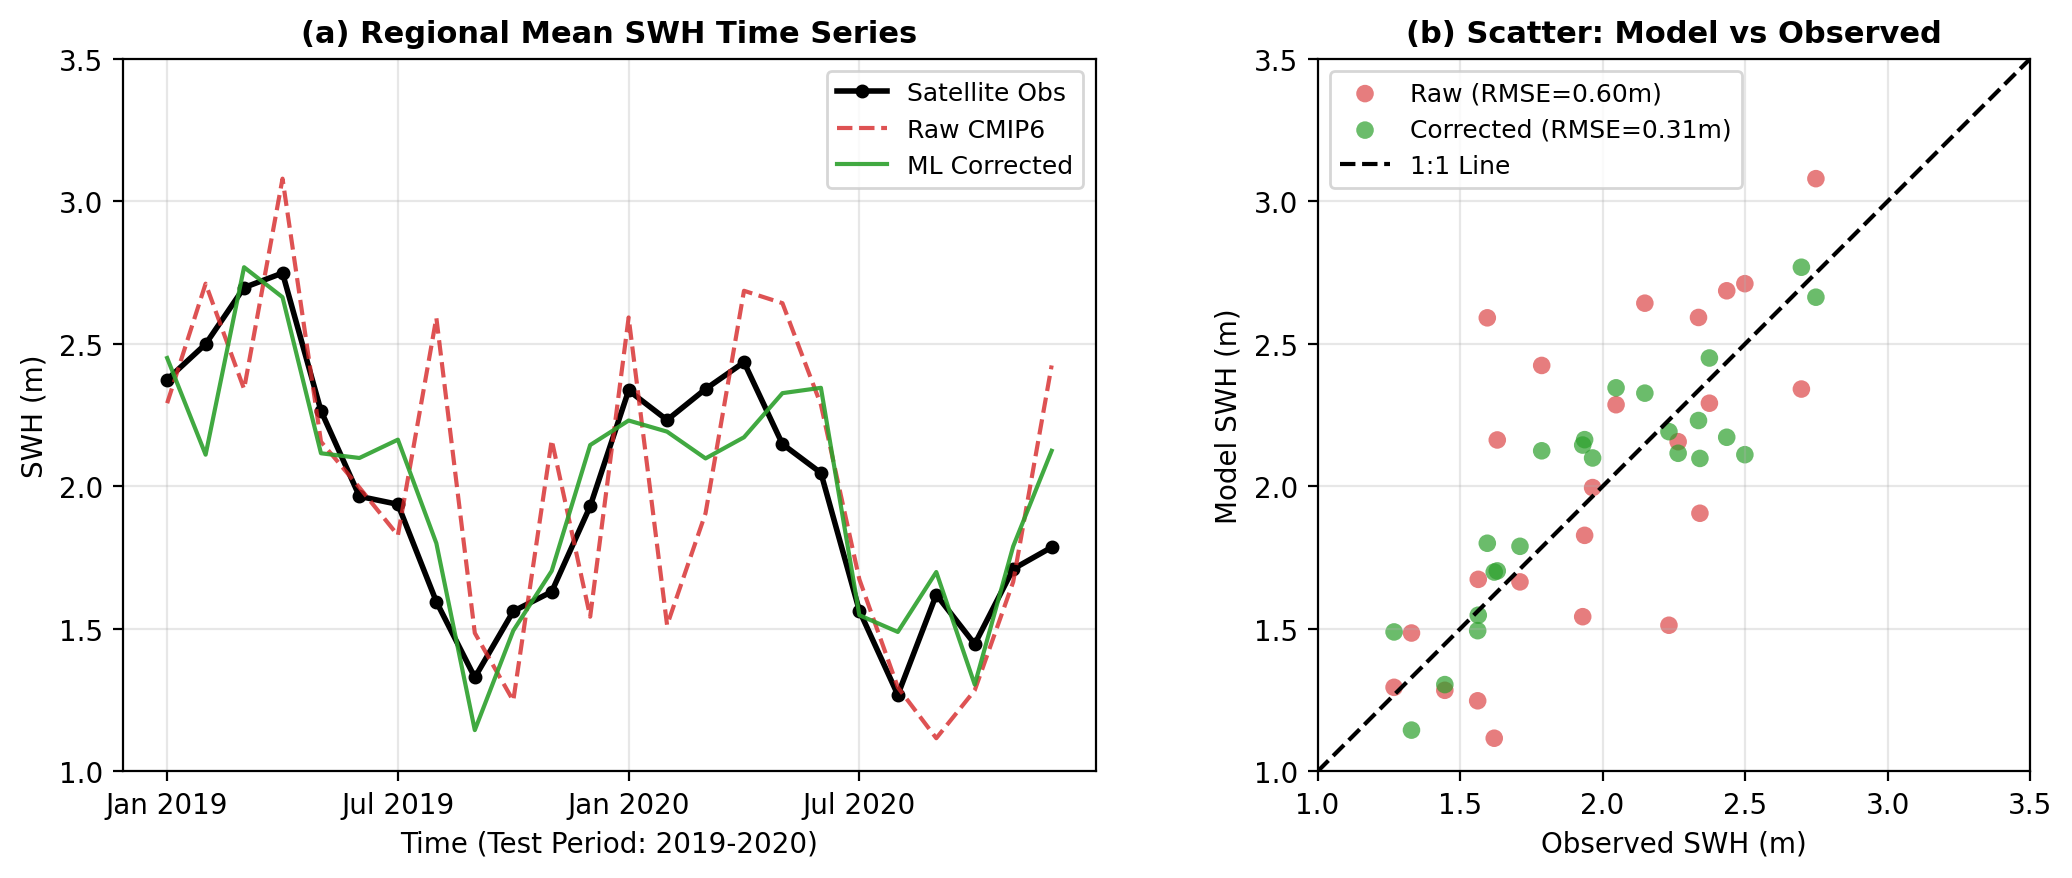
\includegraphics[width=0.95\textwidth]{swh_results_combined.png}
\end{frame}

\begin{frame}{SWH Pilot: Spatial Error Structure}
  \begin{columns}[T,onlytextwidth]
    \column{0.5\textwidth}
      \centering
      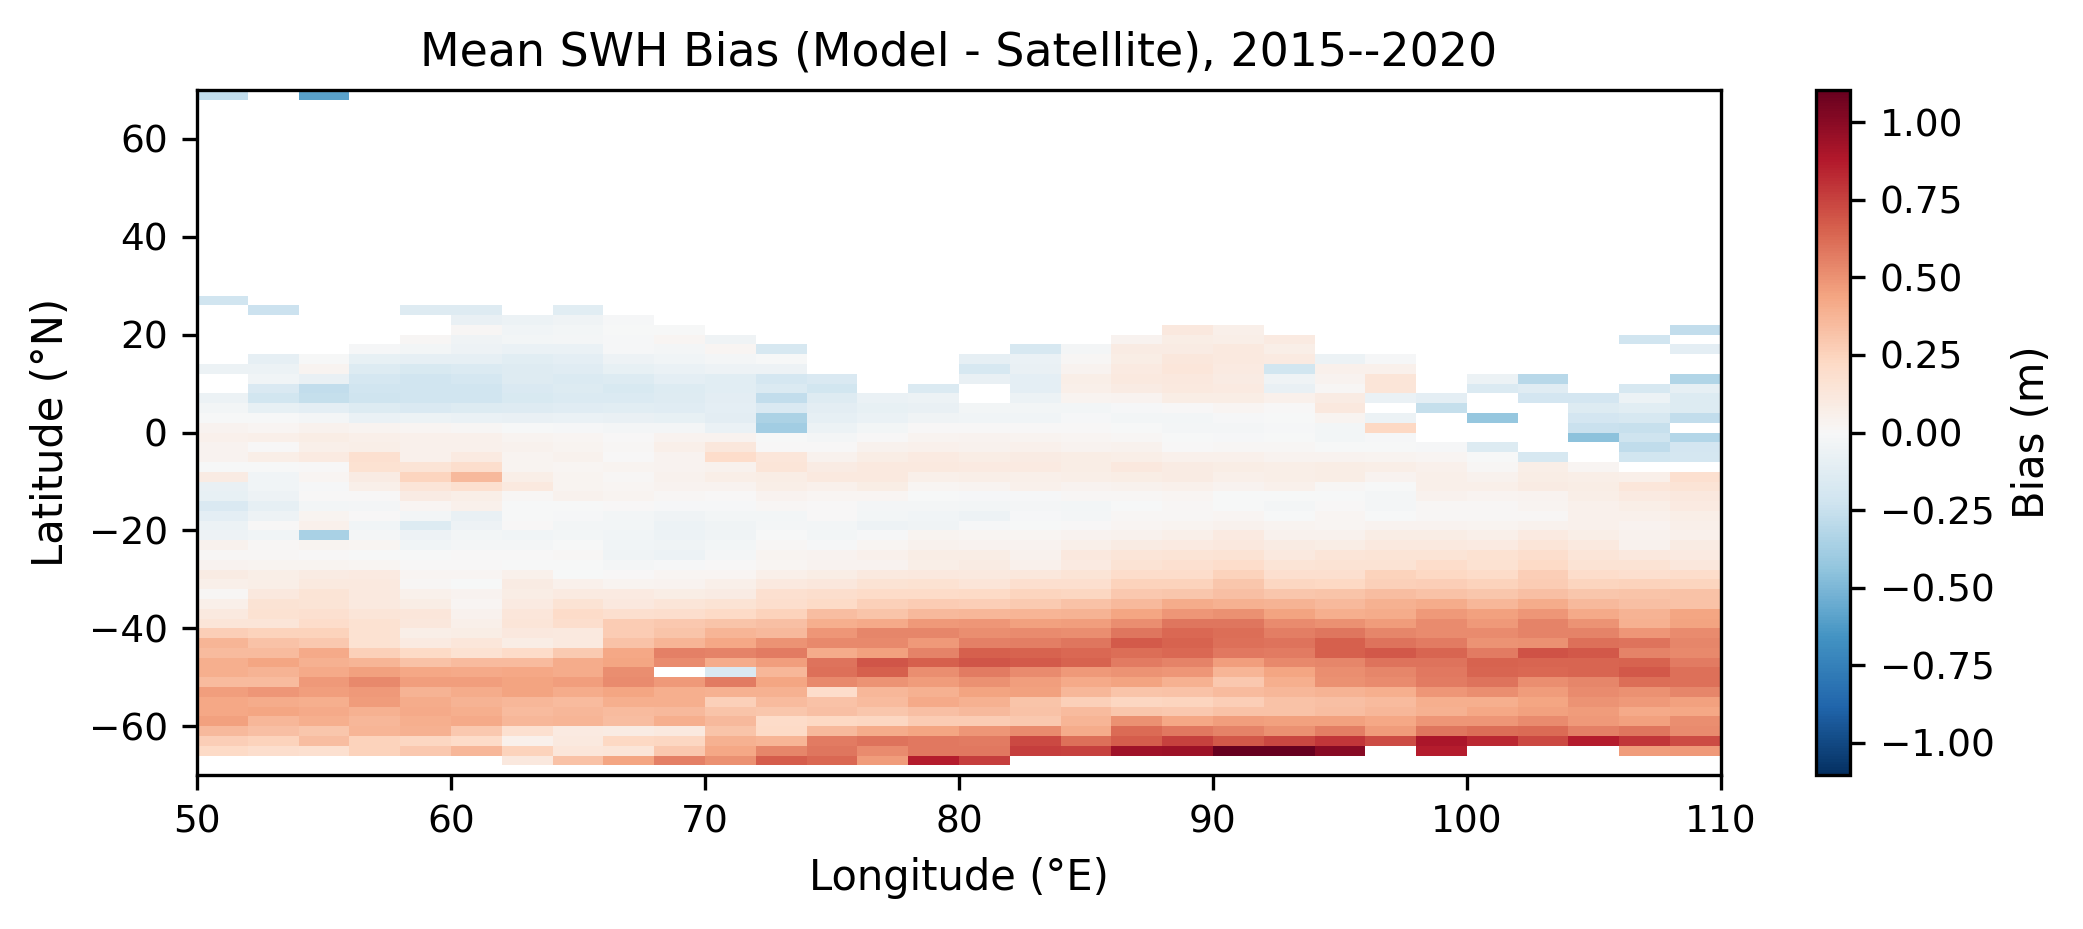
\includegraphics[width=\linewidth,height=0.70\textheight,keepaspectratio]{bias_map.png}
      \vspace{0.25em}

      \footnotesize Baseline bias map (CMIP6 -- altimetry).
    \column{0.5\textwidth}
      \centering
      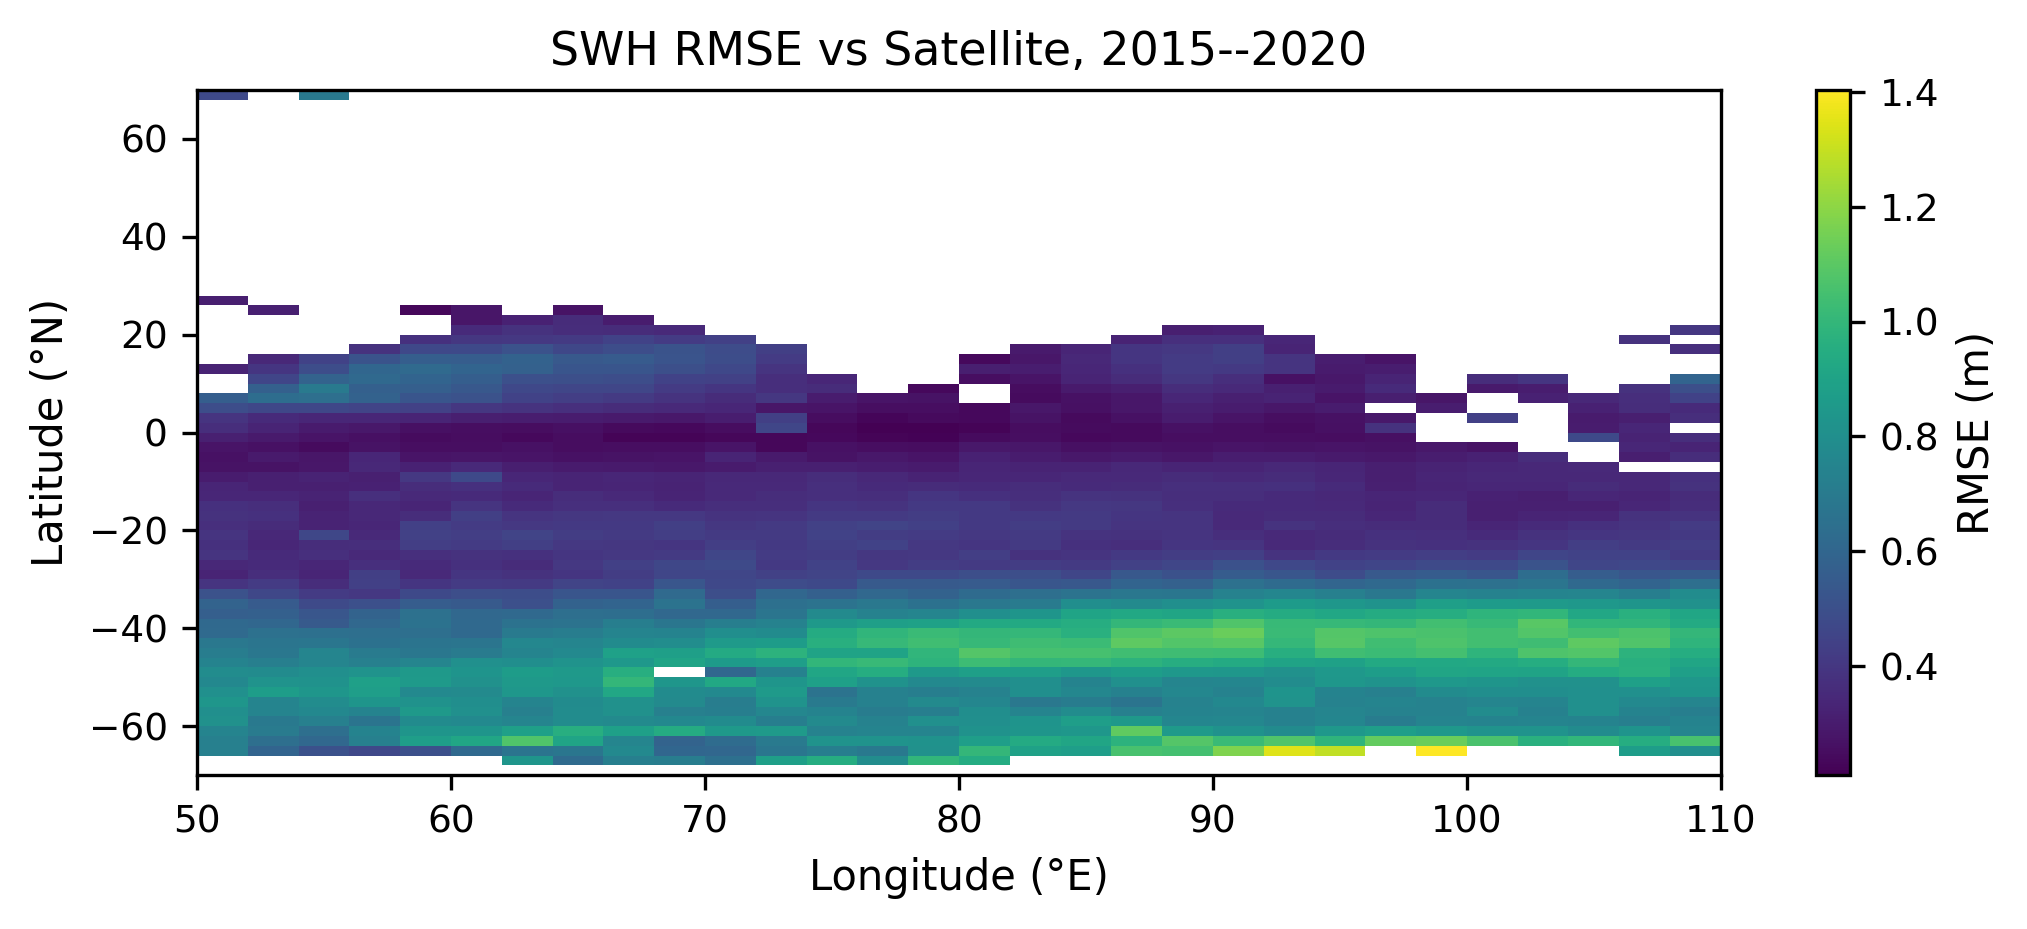
\includegraphics[width=\linewidth,height=0.70\textheight,keepaspectratio]{rmse_map.png}
      \vspace{0.25em}

      \footnotesize Baseline RMSE map.
  \end{columns}
\end{frame}

\begin{frame}{SWH Pilot: Scatter and Time-Series Diagnostics}
  \begin{columns}[T,onlytextwidth]
    \column{0.5\textwidth}
      \centering
      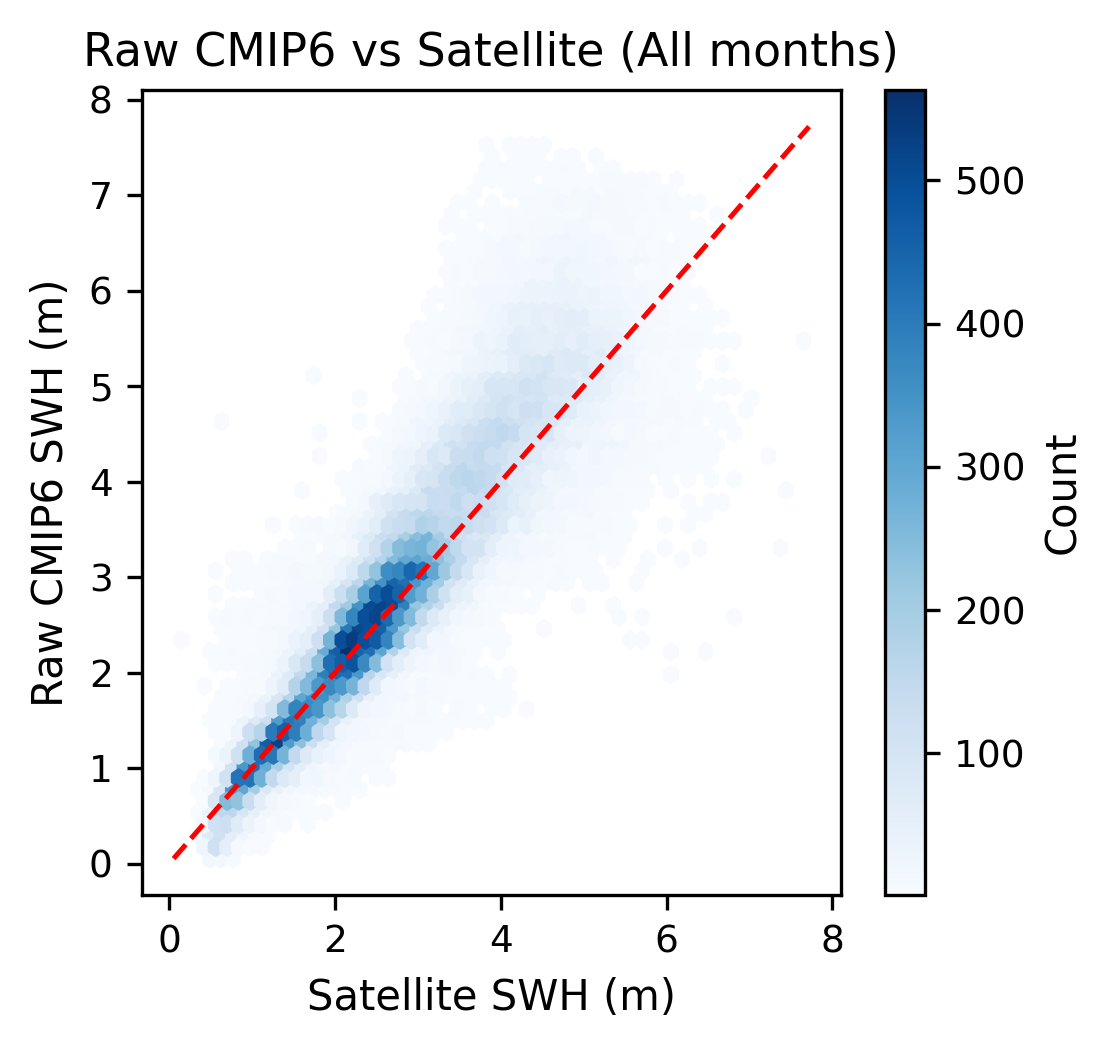
\includegraphics[width=\linewidth,height=0.72\textheight,keepaspectratio]{scatter.png}
      \vspace{0.25em}

      \footnotesize Scatter: raw vs corrected against altimetry.
    \column{0.5\textwidth}
      \centering
      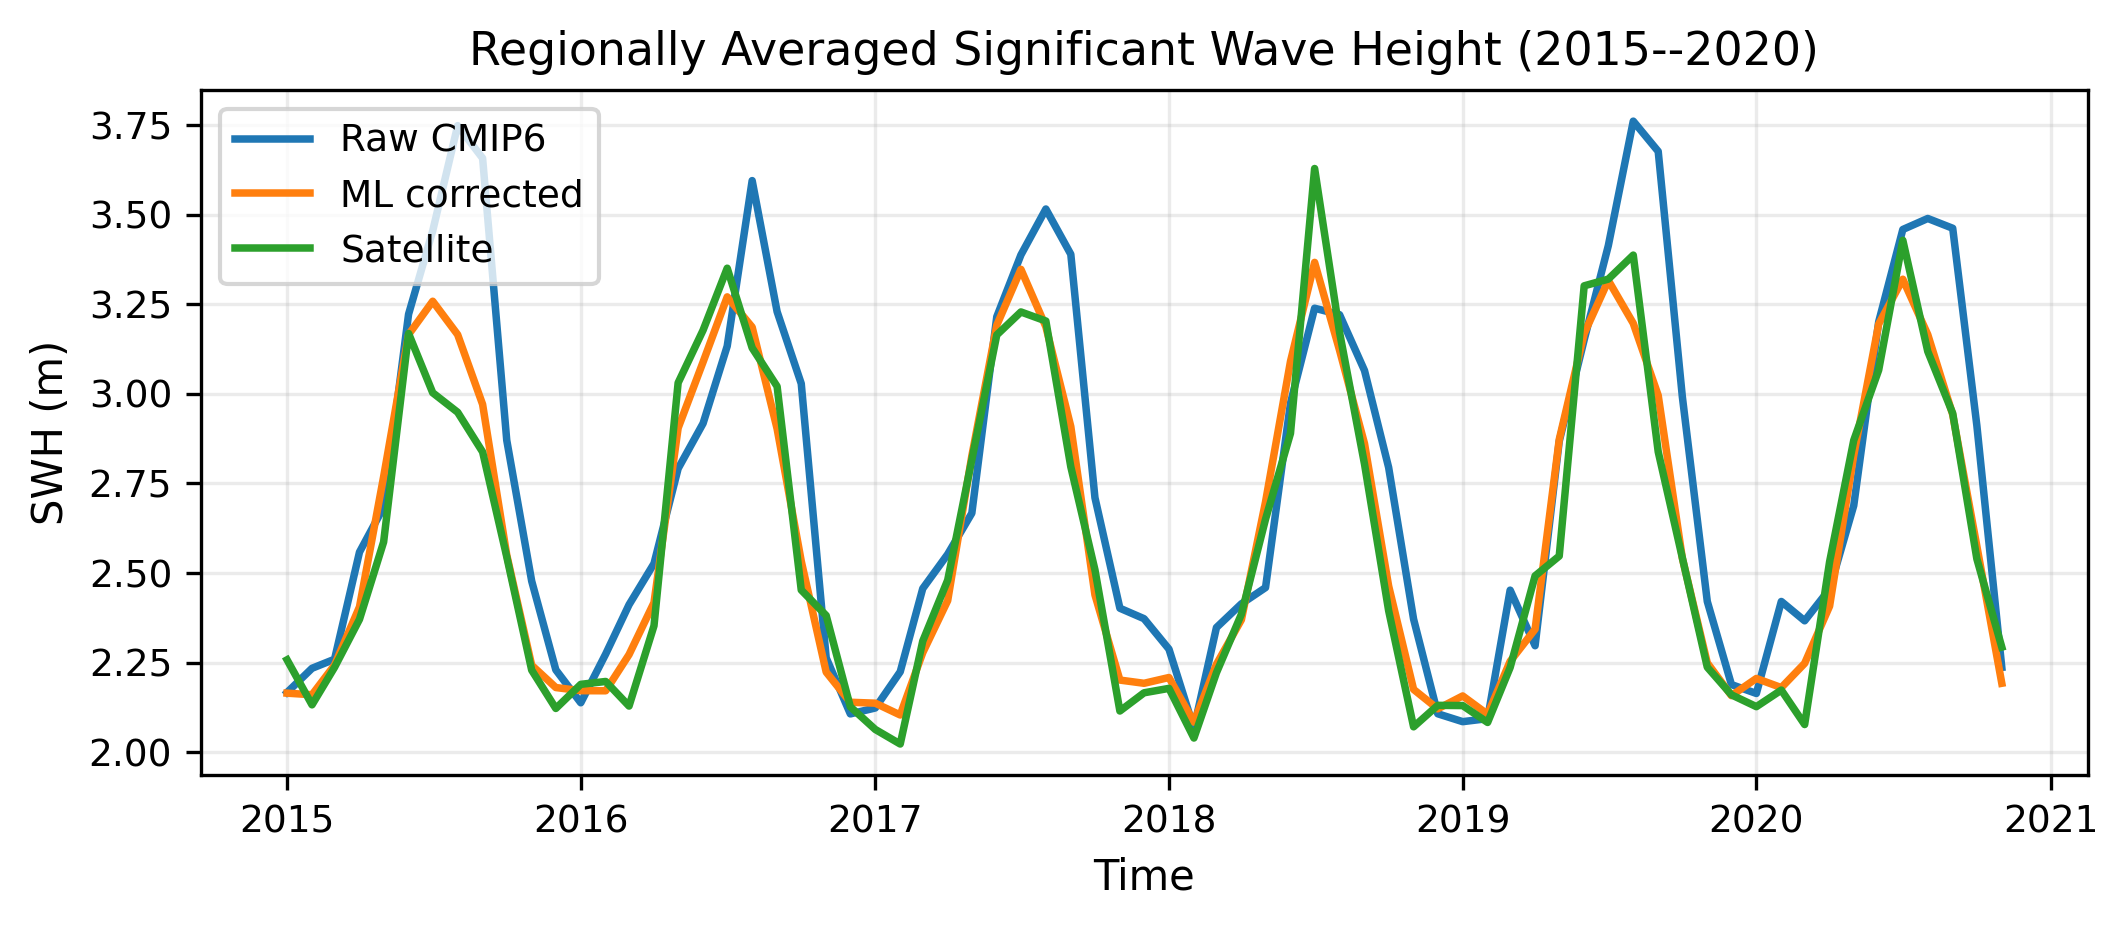
\includegraphics[width=\linewidth,height=0.72\textheight,keepaspectratio]{time_series.png}
      \vspace{0.25em}

      \footnotesize Regional mean time series comparison.
  \end{columns}
\end{frame}

\begin{frame}{SWH Pilot: Seasonality and Distribution Checks}
  \begin{columns}[T,onlytextwidth]
    \column{0.5\textwidth}
      \centering
      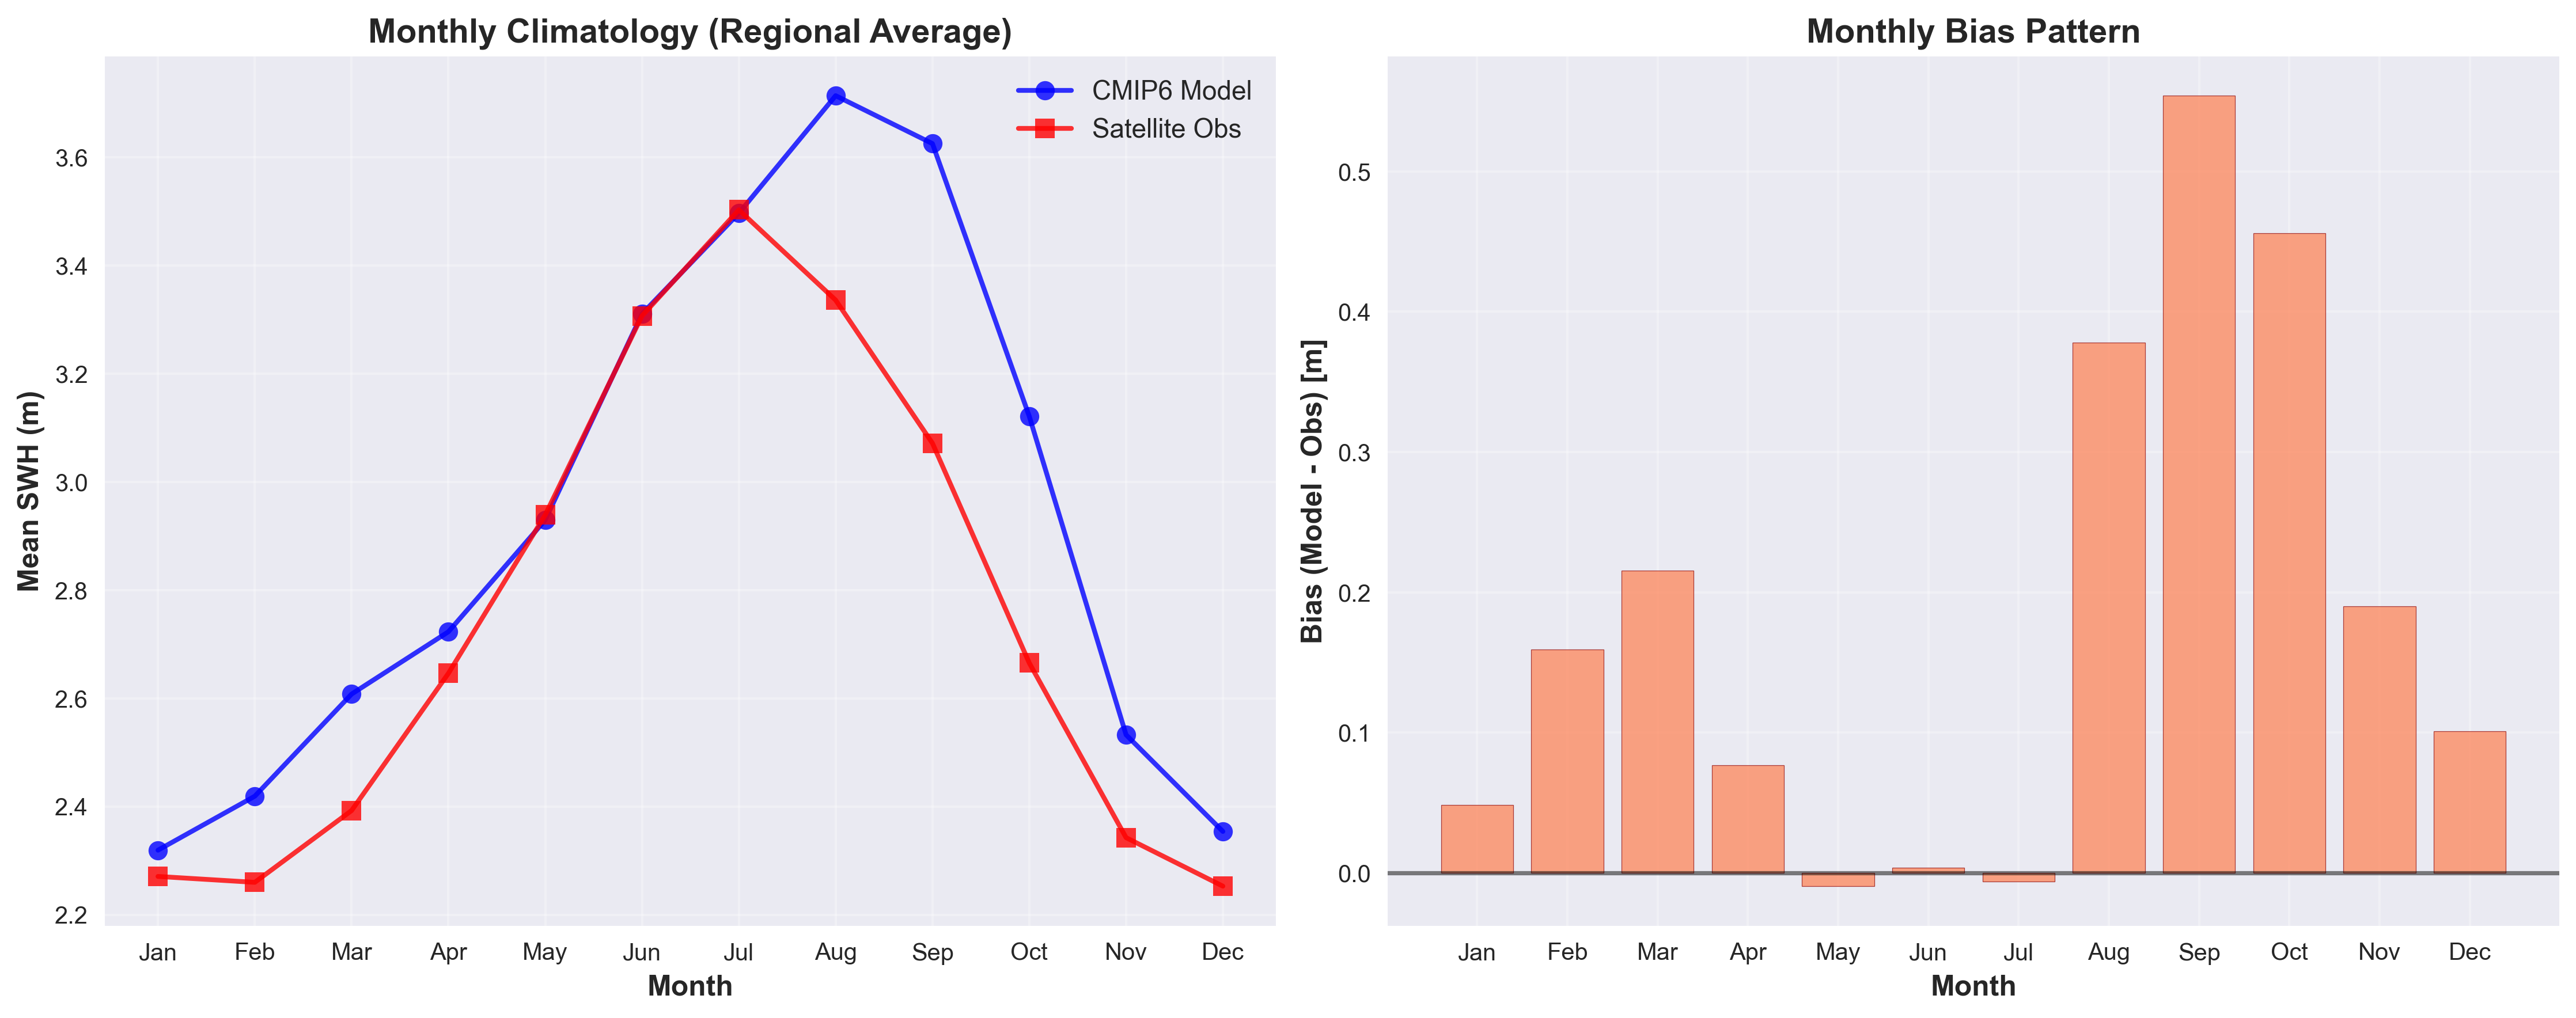
\includegraphics[width=\linewidth,height=0.72\textheight,keepaspectratio]{monthly_climatology.png}
      \vspace{0.25em}

      \footnotesize Monthly climatology and seasonal bias.
    \column{0.5\textwidth}
      \centering
      
\includegraphics[width=\linewidth,height=0.72\textheight,keepaspectratio]{statistical_distributions.png}
      \vspace{0.25em}

      \footnotesize Distribution shift and quantile behaviour.
  \end{columns}
\end{frame}

\begin{frame}{SWH Pilot: Feature Importance}
  \begin{table}
    \centering
    \begin{tabular}{l r}
      \toprule
      Feature & Importance \\
      \midrule
      CMIP6 SWH value & 88.10\% \\
      Latitude & 4.68\% \\
      Month & 4.07\% \\
      Longitude & 3.15\% \\
      \bottomrule
    \end{tabular}
  \end{table}
  \vspace{0.75em}
  \begin{itemize}
    \item Interpretation: most explainable variance is captured by the raw CMIP6 SWH, with geography and seasonality adding spatial/temporal structure.
  \end{itemize}
\end{frame}

\begin{frame}{SLA Pilot: Correction Results}
  \begin{itemize}
    \item Curvilinear-grid handling validated via nearest-neighbour alignment using KD-tree based mapping.
    \item RMSE reduction: 0.1037 m (raw) $\rightarrow$ 0.0578 m (corrected), \textbf{44.3\%} reduction in error variance.
    \item Global SLA baseline trend (2015--2024 mean rate): CMIP6 $\approx$ 3.6 mm/yr vs altimetry $\approx$ 3.3 mm/yr (preliminary).
  \end{itemize}
  \vspace{0.5em}
  \centering
  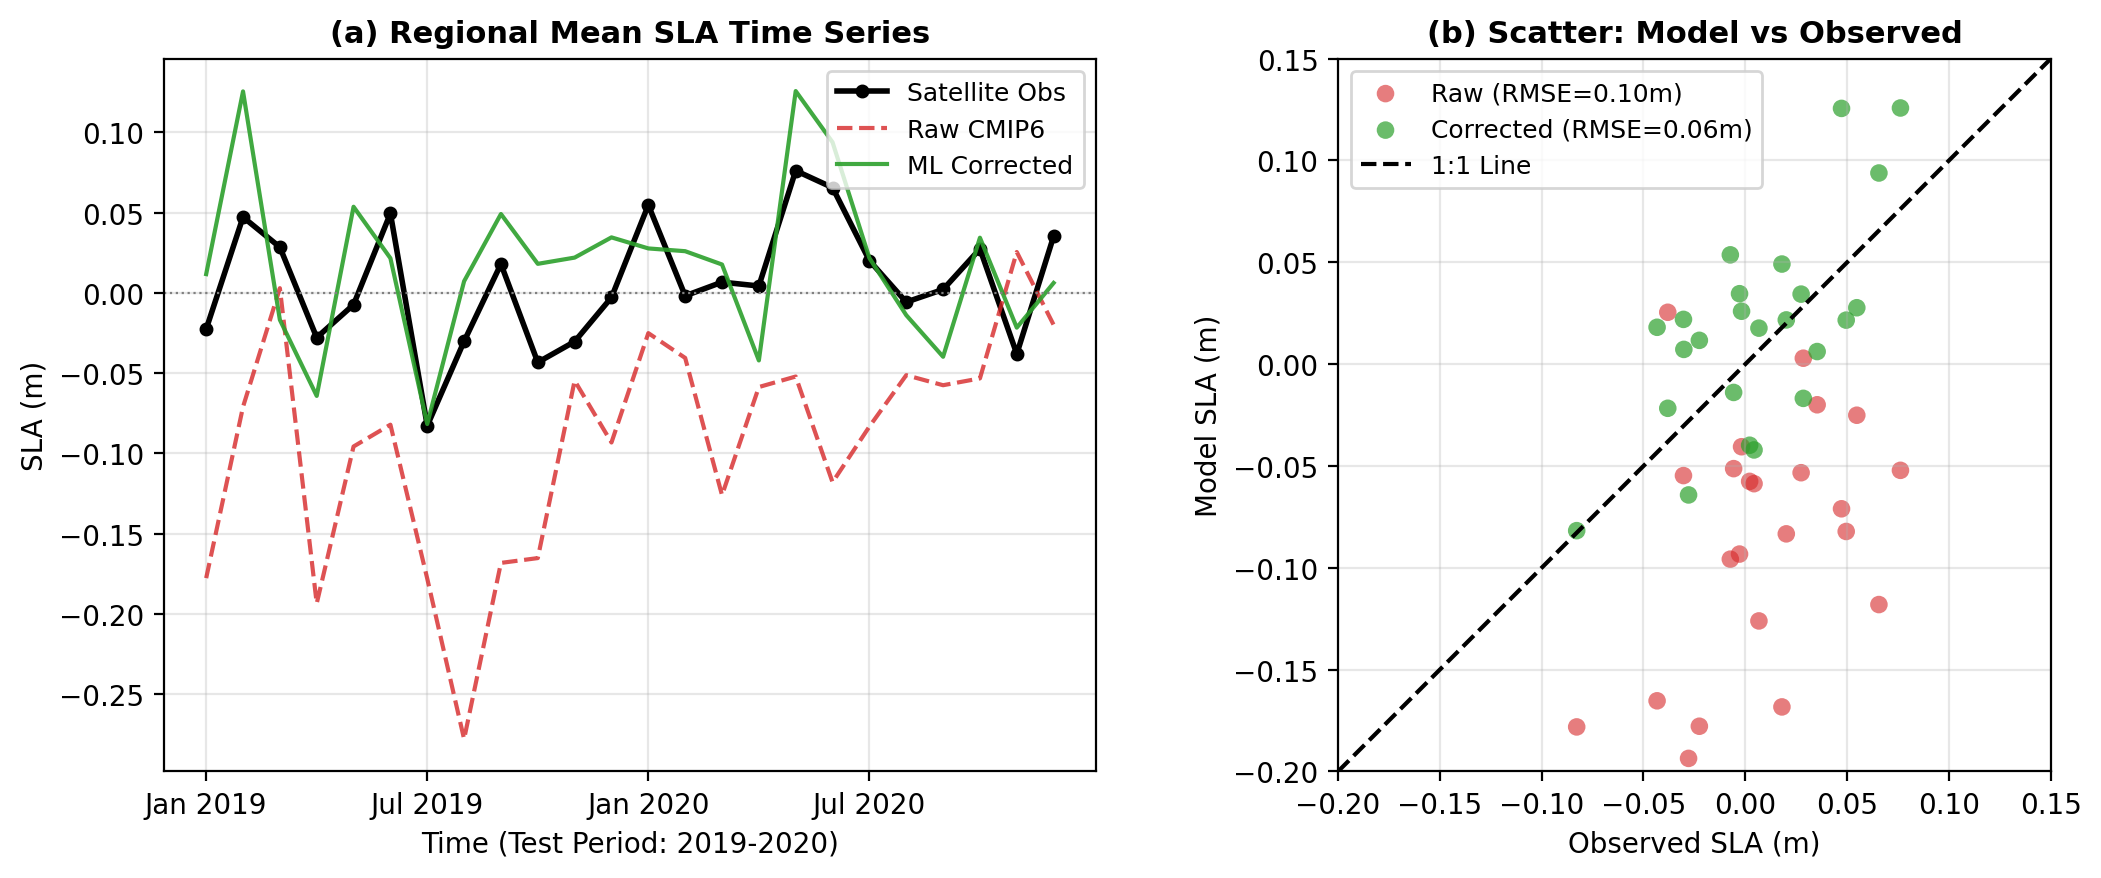
\includegraphics[width=0.95\textwidth]{sla_results_combined.png}
\end{frame}

\begin{frame}{SLA Pilot: Bias Patterns and Time-Series}
  \begin{columns}[T,onlytextwidth]
    \column{0.5\textwidth}
      \centering
      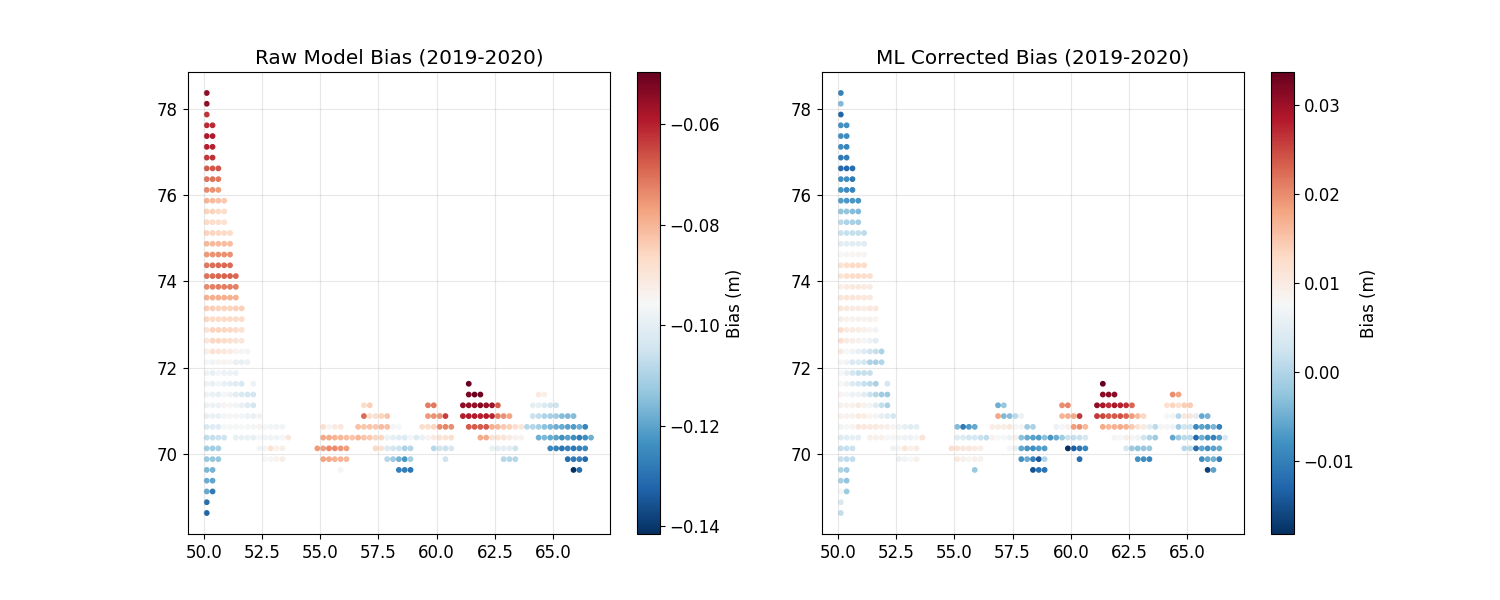
\includegraphics[width=\linewidth,height=0.72\textheight,keepaspectratio]{bias_maps_sla.png}
      \vspace{0.25em}

      \footnotesize Spatial bias structure (pilot region).
    \column{0.5\textwidth}
      \centering
      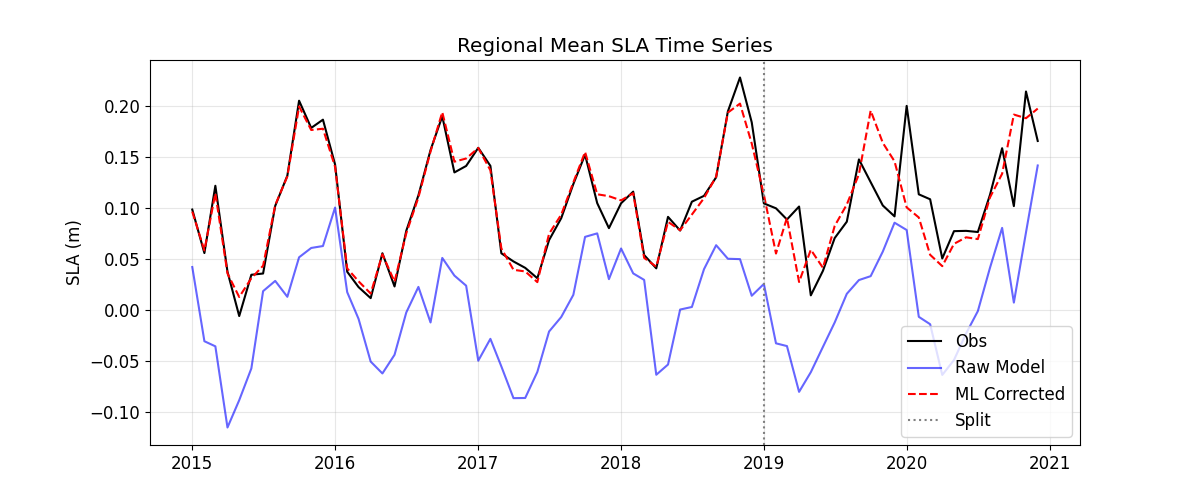
\includegraphics[width=\linewidth,height=0.72\textheight,keepaspectratio]{time_series_sla.png}
      \vspace{0.25em}

      \footnotesize Time series: raw vs corrected against altimetry.
  \end{columns}
\end{frame}

\section{Work Proposed During the Next Year}

\begin{frame}{Work Proposed During the Next Year}
  \begin{itemize}
    \item Scale preprocessing and correction to full observed overlap window (2015--2023) and expand spatial scope to global basins.
    \item Implement uncertainty-aware/probabilistic correction models (QRNN/DeepAR/BNN, ensembles) with spatial/temporal block cross-validation.
    \item Extend SLA bias analysis and correction; validate using tide gauges and extreme-event cases.
    \item Apply validated models to SSP projections and generate corrected products with uncertainty layers for dissemination.
    \item Prepare MOSDAC-ready datasets, metadata, and user documentation/training materials.
  \end{itemize}
\end{frame}

\section{Conclusion}

\begin{frame}{Conclusion}
  \begin{itemize}
    \item A reproducible end-to-end pipeline for QC, co-location/regridding, and ML correction has been established.
    \item SWH pilot demonstrates substantial skill improvement (RMSE: 0.599 m $\rightarrow$ 0.308 m) over the Indian Ocean.
    \item SLA pilot confirms workflow robustness under curvilinear grids and yields strong error reductions (RMSE: 0.1037 m $\rightarrow$ 0.0578 m).
    \item Next steps focus on scaling globally and delivering uncertainty-aware corrected products for MOSDAC distribution.
  \end{itemize}
\end{frame}

\section{References}

\begin{frame}[allowframebreaks]{References}
  \footnotesize
  \begin{thebibliography}{99}
    \bibitem{breiman2001} L. Breiman, ``Random forests,'' \emph{Machine Learning}, 45(1), 2001.
    \bibitem{cannon2018} A. J. Cannon, ``Multivariate quantile mapping bias correction,'' \emph{Climate Dynamics}, 50, 2018.
    \bibitem{lemos2020} G. Lemos et al., ``On the need of bias correction methods for wave climate projections,'' \emph{Global and Planetary Change}, 186, 2020.
    \bibitem{sun2022} D. Sun et al., ``A deep learning-based bias correction method for predicting ocean surface waves,'' \emph{Geophysical Research Letters}, 49(23), 2022.
    \bibitem{duacs} CMEMS/AVISO DUACS products (SLA and related variables), \url{https://www.aviso.altimetry.fr/}.
    \bibitem{cmip6} ESGF CMIP6 archive, \url{https://esgf-node.llnl.gov/projects/cmip6/}.
  \end{thebibliography}
\end{frame}

\end{document}
